\documentclass[../Práctica.root.tex]{subfiles}

\begin{document}

\section{Unidad 4}

\begin{enumerate}
  \item Una pelota se mueve en línea recta (eje $x$). En la gráfica muestra la velocidad de la pelota en función del tiempo.

        \begin{enumerate}
          \item ¿Cuáles son la rapidez media y la velocidad media de la pelota durante los primeros \SI{3,00}{\second}?

                \begin{center}
                  \begin{tabular}{|c|c|} \hline
                    $t$                & $V$                           \\ \hline
                    \SI{2,00}{\second} & \SI{2,00}{\meter\per\second} \\ \hline
                    \SI{1,00}{\second} & \SI{3,00}{\meter\per\second} \\ \hline
                  \end{tabular}
                \end{center}

                \[
                  V_{p_x}
                  =\frac{\sum(t_n\cdot V_n)}{\sum t_n}
                  =\frac{\SI{7,00}{\meter}}{\SI{3,00}{\second}}
                  =\boxed{\SI{2,33}{\meter\per\second}}
                \]
                \[
                  R_p
                  =\frac{\sum(t_n\cdot |V_n|)}{\sum t_n}
                  =\frac{\SI{7,00}{\meter}}{\SI{3,00}{\second}}
                  =\boxed{\SI{2,33}{\meter\per\second}}
                \]

          \item Suponga que la pelota se mueve de tal manera que el segmento de la gráfica después de \SI{2,00}{\second} es de \SI{-3,00}{\meter\per\second} en lugar de \SI{+3,00}{\meter\per\second}. En este caso calcule la rapidez y la velocidad media de la pelota.

                \begin{center}
                  \begin{tabular}{|c|c|} \hline
                    $t$                & $V$                            \\ \hline
                    \SI{2,00}{\second} & \SI{2,00}{\meter\per\second}  \\ \hline
                    \SI{1,00}{\second} & \SI{-3,00}{\meter\per\second} \\ \hline
                  \end{tabular}
                \end{center}

                \[
                  V_{p_x}
                  =\frac{\sum(t_n\cdot V_n)}{\sum t_n}
                  =\frac{\SI{1,00}{\meter}}{\SI{3,00}{\second}}
                  =\boxed{\SI{0,33}{\meter\per\second}}
                \]
                \[
                  R_p
                  =\frac{\sum(t_n\cdot |V_n|)}{\sum t_n}
                  =\frac{\SI{7,00}{\meter}}{\SI{3,00}{\second}}
                  =\boxed{\SI{2,33}{\meter\per\second}}
                \]
        \end{enumerate}

  \item Un automóvil de prueba viaja en linea recta a lo largo del eje $x$. La gráfica indica la posición $x$ del automóvil en función del tiempo. Obtenga la velocidad instantánea en cada uno de los puntos $A$ a $F$.

        \begin{itemize}
          \item Segmento $\alpha$:

                \[
                  V_A=V_B
                  =\frac{\Delta x}{\Delta t}
                  =\frac{x_f-x_i}{t_f-t_i}
                  =\frac{\SI{40,0}{\meter}-\SI{20,0}{\meter}}{\SI{3,00}{\second}-\SI{0,00}{\second}}
                  =\boxed{\SI{6,67}{\meter\per\second}}
                \]

          \item Segmento $\beta$:

                \[
                  V_C
                  =\frac{\Delta x}{\Delta t}
                  =\frac{x_f-x_i}{t_f-t_i}
                  =\frac{\SI{40,0}{\meter}-\SI{40,0}{\meter}}{\SI{5,00}{\second}-\SI{3,00}{\second}}
                  =\boxed{\SI{0,00}{\meter\per\second}}
                \]

          \item Segmento $\gamma$:

                \begin{multicols}{2}
                  \[x(t)=a(t-\SI{6,00}{\second})(t-\SI{9,00}{\second})\]
                  \[\SI{40,0}{\meter}=a(\SI{5,00}{\second}-\SI{6,00}{\second})(\SI{5,00}{\second}-\SI{9,00}{\second})\]
                  \[\SI{40,0}{\meter}=a\cdot\SI{4,00}{\second\squared}\]
                  \[a=\SI{10,0}{\meter\per\second\squared}\]

                  \[x'(t)=v(t)=(\SI{10,0}{\meter\per\second\squared}(t-\SI{6,00}{\second})(t-\SI{9,00}{\second}))'\]
                  \[v(t)=(\SI{10,0}{\meter\per\second\squared}(t^2-\SI{6,00}{\second}t-\SI{9,00}{\second}t+\SI{54,0}{\second\squared})'\]
                  \[v(t)=(\SI{10,0}{\meter\per\second\squared}(t^2-\SI{15,0}{\second}t+\SI{54,0}{\second\squared})'\]
                  \[v(t)=(\SI{10,0}{\meter\per\second\squared}t^2-\SI{150}{\meter\per\second}t+\SI{540}{\meter})'\]
                  \[v(t)=\SI{20,0}{\meter\per\second\squared}t-\SI{150}{\meter\per\second}\]

                  \[V_D=\SI{20,0}{\meter\per\second\squared}\cdot\SI{5,50}{\second}-\SI{150}{\meter\per\second}=\boxed{\SI{-40,0}{\meter\per\second}}\]
                  \[V_E=\SI{20,0}{\meter\per\second\squared}\cdot\SI{6,00}{\second}-\SI{150}{\meter\per\second}=\boxed{\SI{-30,0}{\meter\per\second}}\]
                  \[V_F=\SI{20,0}{\meter\per\second\squared}\cdot\SI{7,50}{\second}-\SI{150}{\meter\per\second}=\boxed{\SI{0,00}{\meter\per\second}}\]
                \end{multicols}
        \end{itemize}

  \item Un antílope que viene corriendo con aceleración constante tarda \SI{7,00}{\second} en pasar por dos puntos que se encuentran separados entre sí \SI{70,0}{\meter}. Su rapidez al pasar por el segundo punto es \SI{15,0}{\meter\per\second}.

        \begin{enumerate}
          \item ¿Qué rapidez tenía al pasar por el primer punto?
          \item ¿Qué aceleración lleva?

                \[x=x_i+V_it+\frac{1}{2}at^2\]
                \[\SI{70,0}{\meter}=V_i\cdot\SI{7,00}{\second}+\frac{1}{2}a\cdot(\SI{7,00}{\second})^2\]

                \[V_f=V_i+at\]
                \[\SI{15,0}{\meter\per\second}=V_i+a\cdot\SI{7,00}{\second}\]
                \[\SI{15,0}{\meter\per\second}-a\cdot\SI{7,00}{\second}=V_i\]

                \[\SI{70,0}{\meter}=(\SI{15,0}{\meter\per\second}-a\cdot\SI{7,00}{\second})\cdot\SI{7,00}{\second}+\frac{1}{2}a\cdot(\SI{7,00}{\second})^2\]
                \[\SI{70,0}{\meter}=\SI{105}{\meter}-a\cdot\SI{49,0}{\second\squared}+a\cdot\SI{24,5}{\second}^2\]
                \[\SI{70,0}{\meter}=\SI{105}{\meter}-a\cdot\SI{24,5}{\second\squared}\]
                \[\SI{-35,0}{\meter}=-a\cdot\SI{24,5}{\second\squared}\]
                \[a=\boxed{\SI{1,43}{\meter\per\second\squared}}\]

                \[V_i=\SI{15,0}{\meter\per\second}-a\cdot\SI{7,00}{\second}=\boxed{\SI{4,99}{\meter\per\second}}\]
        \end{enumerate}

  \item Un malabarista arroja un cuchillo verticalmente hacia arriba con una velocidad inicial de \SI{8,20}{\meter\per\second}. ¿Cuánto tiempo transcurre hasta que el cuchillo regresa a la mano del malabarista?

        \[y=y_i+v_it+\frac{1}{2}at^2\]
        \[0=0+\SI{8,20}{\meter\per\second}t+\frac{1}{2}\cdot\SI{-9,80}{\meter\per\second\squared}t^2\]
        \[0=-\SI{4,90}{\meter\per\second\squared}t^2+\SI{8,20}{\meter\per\second}t+0\]

        \[\{x_1,x_2\}=\frac{-b\pm\sqrt{b^2-4ac}}{2a}\]
        \[\{t_1,t_2\}=\frac{\SI{-8,20}{\meter\per\second}\pm\sqrt{(\SI{8,20}{\meter\per\second})^2-4\cdot-\SI{4,90}{\meter\per\second\squared}\cdot 0}}{2\cdot-\SI{4,90}{\meter\per\second\squared}}\]
        \[\{t_1,t_2\}=\frac{\SI{-8,20}{\meter\per\second}\pm\SI{8,20}{\meter\per\second}}{-\SI{9,80}{\meter\per\second\squared}}\]
        \[t_1=\frac{\SI{-8,20}{\meter\per\second}+\SI{8,20}{\meter\per\second}}{-\SI{9,80}{\meter\per\second\squared}}=0\]
        \[t_2=\frac{\SI{-8,20}{\meter\per\second}-\SI{8,20}{\meter\per\second}}{-\SI{9,80}{\meter\per\second\squared}}=\boxed{\SI{1,67}{\second}}\]

  \item Una pelota de tenis en Marte, donde la aceleración debida a la gravedad es de \SI{3,71}{\meter\per\second\squared} y la resistencia del aire es despreciable, es golpeada directamente hacia arriba y regresa al mismo nivel \SI{8,50}{\second} más tarde.

        \begin{enumerate}
          \item ¿A qué altura del punto original llega la pelota?

                \[y=y_i+v_it+\frac{1}{2}at^2\]
                \[y=\frac{1}{2}\cdot\SI{-3,71}{\meter\per\second\squared}(t)(t-\SI{8,50}{\second})\]
                \[y=\SI{-1,86}{\meter\per\second\squared}\left(\frac{\SI{8,50}{\second}}{2}\right)\left(\frac{\SI{8,50}{\second}}{2}-\SI{8,50}{\second}\right)\]
                \[y=\SI{-1,86}{\meter\per\second\squared}(\SI{4,25}{\second})(\SI{-4,25}{\second})\]
                \[y=\boxed{\SI{33,6}{\meter}}\]

          \item ¿Qué tan rápido se mueve exactamente después de ser golpeada?

                \[y=y_i+v_it+\frac{1}{2}at^2\]
                \[0=0+v_i\cdot\SI{8,50}{\second}+\frac{1}{2}\cdot\SI{-3,71}{\meter\per\second\squared}\cdot(\SI{8,50}{\second})^2\]
                \[0=v_i\cdot\SI{8,50}{\second}-\SI{134}{\meter}\]
                \[\SI{134}{\meter}=v_i\cdot\SI{8,50}{\second}\]
                \[v_i=\boxed{\SI{15,8}{\meter\per\second}}\]
        \end{enumerate}

  \item Las cucarachas grandes pueden correr a \SI{1,50}{\meter\per\second} en tramos cortos. Suponga que enciende la luz en la cocina de su casa y ve una cucaracha alejándose en línea recta a \SI{1,50}{\meter\per\second}. Si usted estaba \SI{0,90}{\meter} detrás del insecto y se acerca hacia este con una rapidez inicial de \SI{0,80}{\meter\per\second}, ¿qué aceleración constante mínima necesitará para alcanzarlo cuando este haya recorrido \SI{1,20}{\meter}, justo antes de escapar bajo un mueble?

        \[x=vt\]
        \[\SI{1,20}{\meter}=\SI{1,50}{\meter\per\second}t\]
        \[\SI{0,80}{\second}=t\]

        \[x=x_i+v_it+\frac{1}{2}at^2\]
        \[\SI{1,20}{\meter}=\SI{-0,90}{\meter}+\SI{0,80}{\meter\per\second}\cdot\SI{0,80}{\second}+\frac{1}{2}a\cdot(\SI{0,80}{\second})^2\]
        \[\SI{1,20}{\meter}=\SI{-0,26}{\meter}+\SI{0,32}{\second\squared}a\]
        \[\SI{1,46}{\meter}=\SI{0,32}{\second\squared}a\]
        \[a=\boxed{\SI{4,56}{\meter\per\second\squared}}\]

  \item El conductor de un automóvil desea rebasar un camión que viaja a una rapidez constante de \SI{20,0}{\meter\per\second}. Inicialmente, el automóvil también viaja a \SI{20,0}{\meter\per\second} y su paragolpe delantero está \SI{24,0}{\meter} atrás del paragolpes trasero del camión. El automóvil adquiere una aceleración constante de \SI{0,600}{\meter\per\second\squared} y regresa al carril del camión cuando su paragolpe trasero está a \SI{26,0}{\meter} adelante del frente del camión. El automóvil tiene una longitud de \SI{4,50}{\meter}, y el camión tiene una longitud de \SI{21,0}{\meter}.

        \begin{center}
          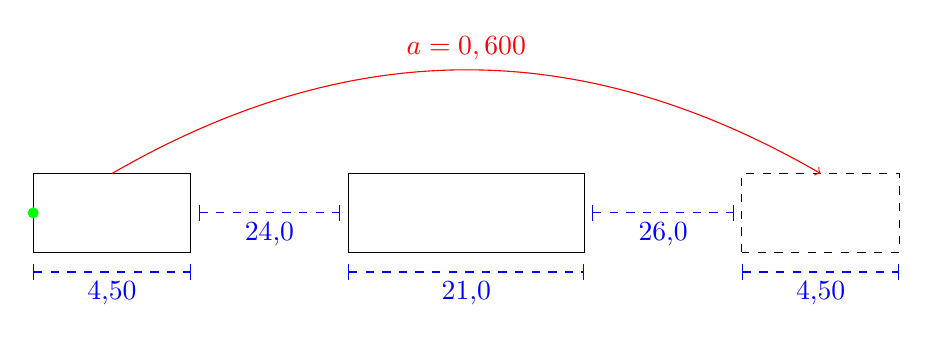
\begin{tikzpicture}
            \draw (0,0) rectangle(2,1);
            \fill[green] (0,0.5) circle(2pt);
            \draw[blue,dashed,|-|] (0,-.25) -- ++(2,0) node[pos=.5,below]{\SI{4,50}{\meter}};
            \draw[blue,dashed,|-|] (2.1,.5) -- ++(1.8,0) node[pos=.5,below]{\SI{24,0}{\meter}};
            \draw (4,0) rectangle(7,1);
            \draw[blue,dashed,|-|] (4,-.25) -- ++(3,0) node[pos=.5,below]{\SI{21,0}{\meter}};
            \draw[blue,dashed,|-|] (7.1,.5) -- ++(1.8,0) node[pos=.5,below]{\SI{26,0}{\meter}};
            \draw[dashed] (9,0) rectangle(11,1);
            \draw[blue,dashed,|-|] (9,-.25) -- ++(2,0) node[pos=.5,below]{\SI{4,50}{\meter}};
            \draw[red,->] (1,1) to[bend left] node[pos=.5,above]{$a=\SI{0,600}{\meter\per\second\squared}$} (10,1);
          \end{tikzpicture}
        \end{center}

        \begin{enumerate}
          \item ¿Cuánto tiempo necesita el automóvil para rebasar al camión?

                \[x_f=x_i+v_it+\frac{1}{2}at^2\]

                Relativo al camion, el automovil esta quieto ($v_i=0$).

                \[\SI{4,50}{\meter}+\SI{24,0}{\meter}+\SI{21,0}{\meter}+\SI{26,0}{\meter}=\frac{1}{2}\cdot\SI{0,600}{\meter\per\second\squared}t^2\]
                \[\SI{75,5}{\meter}=\SI{0,300}{\meter\per\second\squared}t^2\]
                \[\SI{251}{\second\squared}=t^2\]
                \[t=\boxed{\SI{15,8}{\second}}\]

          \item ¿Qué distancia recorre el automóvil ese ese tiempo? ¿Qué rapidez final tiene el automóvil?

                \[x_f=x_i+v_it+\frac{1}{2}at^2\]
                \[x_f=\SI{20,0}{\meter\per\second}\cdot\SI{15,8}{\second}+\frac{1}{2}\cdot\SI{0,600}{\meter\per\second\squared}\cdot(\SI{15,8}{\second})^2\]
                \[x_f=\boxed{\SI{390}{\meter}}\]

                \[v_f=v_i+at\]
                \[v_f=\SI{20,0}{\meter\per\second}+\SI{0,600}{\meter\per\second\squared}\cdot\SI{15,8}{\second}\]
                \[v_f=\boxed{\SI{29,5}{\meter\per\second}}\]
        \end{enumerate}

        \newpage

  \item Se lanza un cohete a escala directamente hacia arriba con una velocidad inicial de \SI{50,0}{\meter\per\second}, y acelera a \SI{2,00}{\meter\per\second\squared} de manera constante hacia arriba hasta que los motores se apagan a una altitud de \SI{150}{\meter}.

        \begin{multicols}{3}
          \begin{center}
            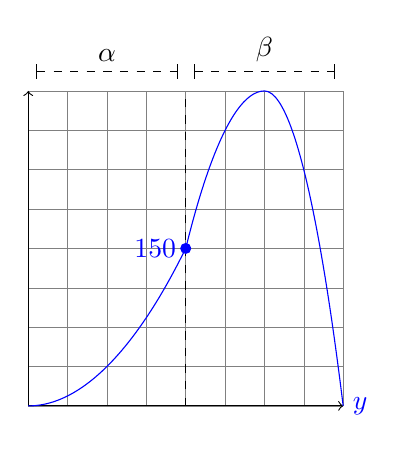
\begin{tikzpicture}
              \draw[help lines, step=.5] (0,0) grid (4,4);
              \draw[->] (0,0) -- (4,0);
              \draw[->] (0,0) -- (0,4);
              \draw[dashed] (2,0) -- ++(0,4);
              \draw[dashed,|-|] (.1,4.25) -- ++(1.8,0) node[pos=.5,above]{$\alpha$};
              \draw[dashed,|-|] (2.1,4.25) -- ++(1.8,0) node[pos=.5,above]{$\beta$};
              \draw[blue] (0,0) parabola (2,2) parabola bend (3,4) (4,0) node[right]{$y$};
              \fill[blue] (2,2) circle(2pt) node[left]{\SI{150}{\meter}};
            \end{tikzpicture}
          \end{center}
          \begin{center}
            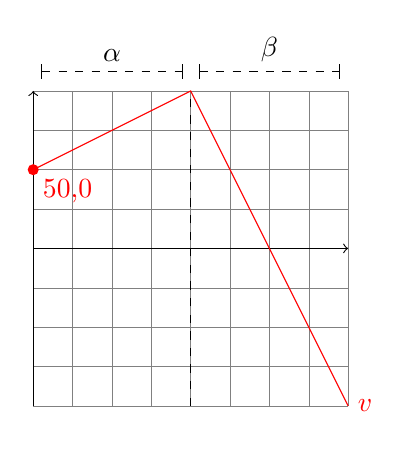
\begin{tikzpicture}
              \draw[help lines, step=.5] (0,0) grid(4,4);
              \draw[->] (0,2) -- ++(4,0);
              \draw[->] (0,0) -- ++(0,4);
              \draw[dashed] (2,0) -- ++(0,4);
              \draw[dashed,|-|] (.1,4.25) -- ++(1.8,0) node[pos=.5,above]{$\alpha$};
              \draw[dashed,|-|] (2.1,4.25) -- ++(1.8,0) node[pos=.5,above]{$\beta$};
              \draw[red] (0,3) -- (2,4) -- (4,0) node[right]{$v$};
              \fill[red] (0,3) circle(2pt) node[below right]{\SI{50,0}{\meter\per\second}};
            \end{tikzpicture}
          \end{center}
          \begin{center}
            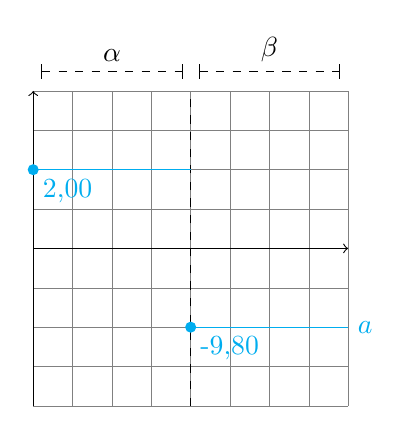
\begin{tikzpicture}
              \draw[help lines, step=.5] (0,0) grid(4,4);
              \draw[->] (0,2) -- (4,2);
              \draw[->] (0,0) -- (0,4);
              \draw[dashed] (2,0) -- ++(0,4);
              \draw[dashed,|-|] (.1,4.25) -- ++(1.8,0) node[pos=.5,above]{$\alpha$};
              \draw[dashed,|-|] (2.1,4.25) -- ++(1.8,0) node[pos=.5,above]{$\beta$};
              \draw[cyan] (0,3) -- (2,3) (2,1) -- (4,1) node[right]{$a$};
              \fill[cyan] (0,3) circle(2pt) node[below right]{\SI{2,00}{\meter\per\second\squared}};
              \fill[cyan] (2,1) circle(2pt) node[below right]{\SI{-9,80}{\meter\per\second\squared}};
            \end{tikzpicture}
          \end{center}
        \end{multicols}

        \begin{enumerate}
          \item ¿Cuál es la altura máxima que alcanza el cohete?

                \begin{multicols}{2}
                  \[y_{\alpha f}=y_{\alpha i}+v_{\alpha i}t+\frac{1}{2}a_\alpha t^2\]
                  \[\SI{150}{\meter}=\SI{50,0}{\meter\per\second}t+\frac{1}{2}\cdot\SI{2,00}{\meter\per\second\squared}t^2\]
                  \[\SI{150}{\meter}=\SI{50,0}{\meter\per\second}t+\SI{1,00}{\meter\per\second\squared}t^2\]
                  \[0=\SI{1,00}{\meter\per\second\squared}t^2+\SI{50,0}{\meter\per\second}t-\SI{150}{\meter}\]

                  \[\{t_1,t_2\}=\frac{-b\pm\sqrt{b^2-4ac}}{2a}\]
                  \[\{t_1,t_2\}=\frac{\SI{-50,0}{\meter\per\second}\pm\sqrt{(\SI{50,0}{\meter\per\second})^2-4\cdot\SI{1,00}{\meter\per\second\squared}\cdot-\SI{150}{\meter}}}{2\cdot\SI{1,00}{\meter\per\second\squared}}\]
                  \[\{t_1,t_2\}=\frac{\SI{-50,0}{\meter\per\second}\pm\SI{55,7}{\meter\per\second}}{\SI{2,00}{\meter\per\second\squared}}\]
                  \[t_1=\SI{2.85}{\second}, t_2=\SI{-52,85}{\second}\]
                  \[t_{\alpha f}=\SI{2.85}{\second}\]

                  \[v_{\beta i}=v_{\alpha i}+a_\alpha t_{\alpha f}\]
                  \[v_{\beta i}=\SI{50,0}{\meter\per\second}+\SI{2,00}{\meter\per\second\squared}\cdot\SI{2.85}{\second}\]
                  \[v_{\beta i}=\SI{55,7}{\meter\per\second}\]

                  \[f(t)=y_{\beta i}+v_{\beta i}t+\frac{1}{2}a_\beta t^2\]
                  \[f(t)=\SI{150}{\meter}+\SI{55,7}{\meter\per\second}t+\frac{1}{2}\cdot\SI{-9,80}{\meter\per\second\squared}t^2\]
                  \[f'(t)=\left(\SI{150}{\meter}+\SI{55,7}{\meter\per\second}t+\frac{1}{2}\cdot\SI{-9,80}{\meter\per\second\squared}t^2\right)'\]
                  \[f'(t)=\SI{55,7}{\meter\per\second}-\SI{9,80}{\meter\per\second\squared}t\]
                  \[0=\SI{55,7}{\meter\per\second}-\SI{9,80}{\meter\per\second\squared}t_{max}\]
                  \[\SI{-55,7}{\meter\per\second}=\SI{-9,80}{\meter\per\second\squared}t_{max}\]
                  \[t_{max}=\SI{5,68}{\second}\]

                  \[y_{max}=y_{\beta i}+v_{\beta i}t_{max}+\frac{1}{2}a_\beta{t_{max}}^2\]
                  \[y_{max}=\SI{150}{\meter}+\SI{55,7}{\meter\per\second}\cdot\SI{5,68}{\second}+\frac{1}{2}\cdot\SI{-9,80}{\meter\per\second\squared}\cdot(\SI{5,68}{\second})^2\]
                  \[y_{max}=\boxed{\SI{308}{\meter}}\]
                \end{multicols}

          \item ¿Cuánto tarda el cohete después de despegue vertical en alcanzar su altura máxima?

                \[t_{\alpha f}+t_{max}=\SI{2.85}{\second}+\SI{5,68}{\second}=\boxed{\SI{8,53}{\second}}\]

                \newpage

          \item ¿Cuánto tarda el cohete en el aire?

                \[y_{\beta f}=y_{\beta i}+v_{\alpha i}t_{\beta f}+\frac{1}{2}a_\alpha{t_{\beta f}}^2\]
                \[0=\SI{150}{\meter}+\SI{55,7}{\meter\per\second}t_{\beta f}+\frac{1}{2}\cdot\SI{-9,80}{\meter\per\second\squared}{t_{\beta f}}^2\]
                \[0=\SI{-4,90}{\meter\per\second\squared}{t_{\beta f}}^2+\SI{55,7}{\meter\per\second}t_{\beta f}+\SI{150}{\meter}\]
                \[\{t_1,t_2\}=\frac{-b\pm\sqrt{b^2-4ac}}{2a}\]
                \[\{t_1,t_2\}=\frac{\SI{-55,7}{\meter\per\second}\pm\sqrt{(\SI{55,7}{\meter\per\second})^2-4\cdot\SI{-4,90}{\meter\per\second\squared}\cdot\SI{150}{\meter}}}{2\cdot\SI{-4,90}{\meter\per\second\squared}}\]
                \[\{t_1,t_2\}=\frac{\SI{-55,7}{\meter\per\second}\pm\SI{77,7}{\meter\per\second}}{\SI{-9,80}{\meter\per\second\squared}}\]
                \[t_1=\SI{-2,24}{\second},t_2=\SI{13,61}{\second}\]
                \[t_{\beta f}=\boxed{\SI{13,61}{\second}}\]
        \end{enumerate}

  \item En la Tierra, una roca de \SI{15,0}{\kilogram} se suelta desde el reposo y llega al suelo en \SI{1,75}{\second}. Cuando se suelta de la misma altura en Encéfalo, una luna de Saturno, llega al suelo en \SI{18,6}{\second}. ¿Cuál es la aceleración debida a la gravedad en Encéfalo?

        \[y_f=y_i+v_it+\frac{1}{2}g_tt^2\]
        \[0=y_i+\frac{1}{2}\cdot\SI{-9,80}{\meter\per\second\squared}(\SI{1,75}{\second})^2\]
        \[0=y_i-\SI{15,0}{\meter}\]
        \[y_i=\SI{15,0}{\meter}\]

        \[y_f=y_i+v_it+\frac{1}{2}g_et^2\]
        \[0=\SI{15,0}{\meter}+\frac{1}{2}g_e(\SI{18,6}{\second})^2\]
        \[\SI{-15,0}{\meter}=\SI{173}{\second\squared}g_e\]
        \[g_e=\boxed{\SI{-0,0867}{\meter\per\second\squared}}\]
\end{enumerate}
\end{document}
